\newpage
\section{Teoria}
\subsection{Modulação AM/DSB}
A modulação em amplitude consiste em modificar a amplitude de um sinal de frequência constante, chamado de portadora, a partir de um sinal modulante (informação). O termo DSB significa \textit{double side band}, pois o espectro do sinal modulado possui tanto a banda positiva quanto a banda negativa do sinal modulante.

O sinal modulado em AM/DSB pode ser representado matematicamente pela equação

\begin{equation}
s(t) = A_c[1+\gamma f(t)]cos(w_c t).
\label{e_am}
\end{equation}

Onde $f(t)$ é o sinal de informação, $A_c$ é a amplitude, $\gamma$ é o índice de modulação e $w_c$ é a frequência angular da portadora.

Sendo 
\[ f(t) = cos(w_m t), \]

temos que
\begin{equation}
s(t) = A_c  \bigg \{ sen(w_c t) + \frac{\gamma}{2}sen(w_c + w_m)t + \frac{\gamma}{2}sen(w_c - w_m)t \bigg  \} .
\label{e_amdsb}
\end{equation}

A transformada de Fourier do sinal da equação \ref{e_amdsb} (mostrada na figura \ref{f_fourier_am_dsb} ) é 
\[
F(s) = \mathfrak{F} \big \{ f(t) \big \} = A_c \delta (s - w_c) + A_c \frac{\gamma}{2}\delta(w_c  + w_m) + A_c \frac{\gamma}{2}\delta(w_c  - w_m)
\]

\begin{figure}[H]
    \centering
    \caption{Modulo do espectro complexo de Fourier da modulação AM DSB com sinal modulante cossenoidal.}
    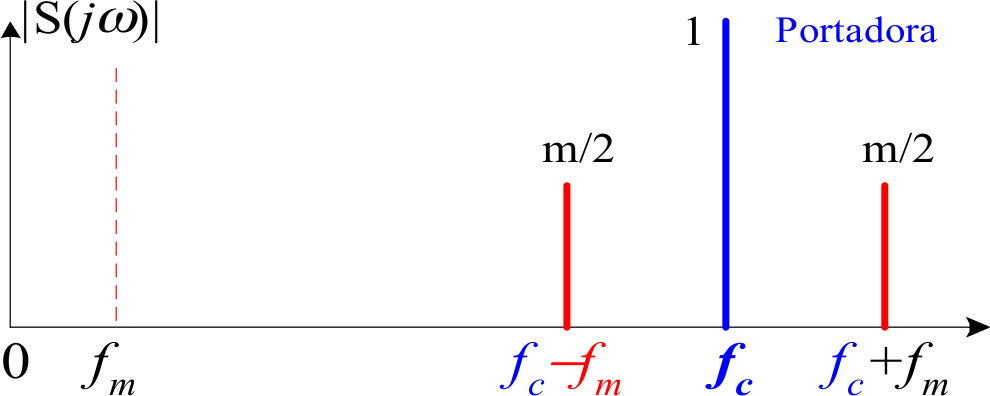
\includegraphics[scale=0.3]{Imagens/fourier_am_dsb.png}
    \label{f_fourier_am_dsb}
\end{figure}


\subsection{Medida do índice de modulação $\bm{\gamma}$}
O índice de modulação ($\gamma$) pode ser obtido através da equação \ref{e_gamma}, onde os valores de \textit{a} e \textit{b} podem ser definidos de duas maneiras.

\begin{equation}
\gamma = \frac{a - b}{a + b}
\label{e_gamma}
\end{equation}

\subsubsection{Método 1}
No método 1, o sinal modulado é colocado no eixo Y e o tempo é colocado no eixo X. O valor de \textit{a} é dado pela amplitude de pico a pico do sinal modulado quando $f(t)$ é máximo e o valor de \textit{b} é dado pelo valor de pico a pico para quando o sinal  $f(t)$ é mínimo. A figura \ref{f_gamma1} mostra um exemplo do cálculo.

\begin{figure}[H]
\centering
\caption{Exemplo para o calculo de $\gamma$, com \textit{a} = 3, \textit{b} = 1 e $\gamma$ = 0.5.}
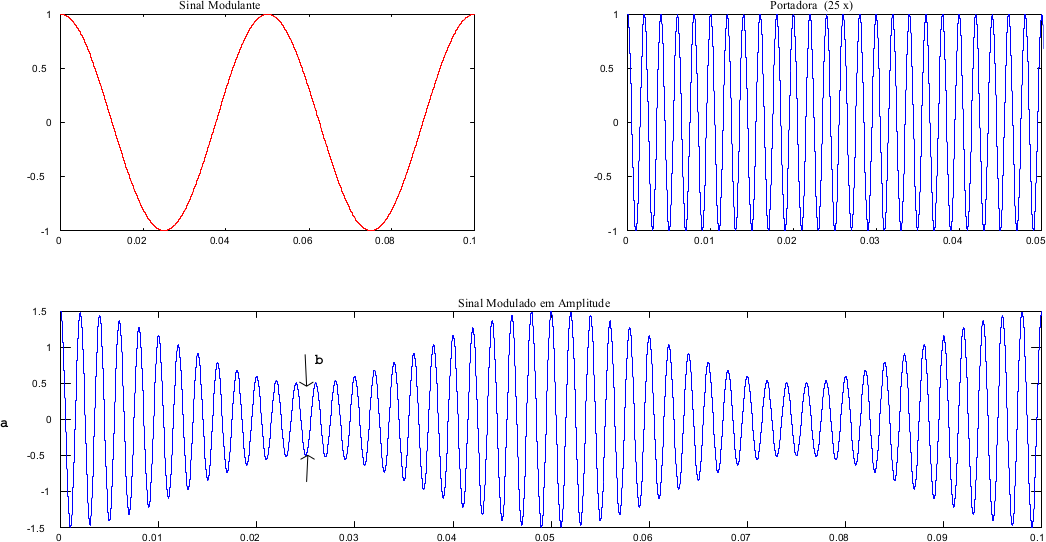
\includegraphics[scale=0.4]{Imagens/gamma1.png}
\label{f_gamma1}
\end{figure}

\subsubsection{Método 2}

No método 2, o sinal modulado é colocado no eixo Y e o sinal modulante é colocado no eixo X. O valor de \textit{a} é dado pela amplitude de pico a pico do da parte mais baixa da figura e o valor de \textit{b} é dado pelo valor de pico a pico mais alto. A figura \ref{f_gamma2} mostra um exemplo do cálculo.

\begin{figure}[H]
    \centering
    \caption{Exemplo para o calculo de $\gamma$, com \textit{a} = 0.2, \textit{b} = 0.6 e $\gamma$ = 0.5.}
    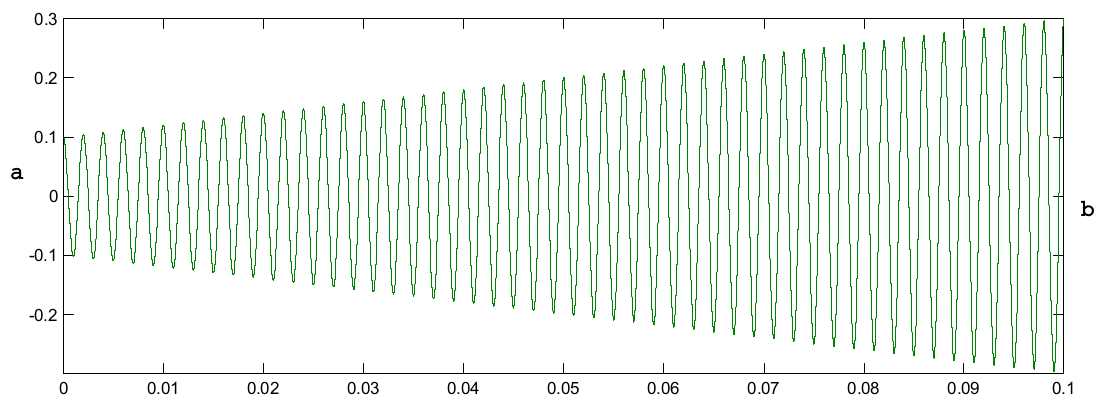
\includegraphics[scale=0.4]{Imagens/gamma2.png}
    \label{f_gamma2}
\end{figure}

O método 2 é preferível, pois evidencia a linearidade do modulador, independente da forma de onda do sinal modulante. Porém, quando são introduzidas distorções no sinal modulado, o método 1 deve ser utilizado.

\subsection{Circuitos moduladores}
Abaixo são apresentadas duas topologias de circuito modulador AM DSB, uma utilizando transistores e a outra empregando um único diodo.

\subsubsection{Modulador série}

A figura \ref{f_mod_am_serie} apresenta a configuração do circuito utilizado em um modulador AM/DSB série.
Os moduladores série modificam diretamente a amplitude do sinal de RF, assim, evitando distorções na frequência do sinal modulado.

O transistor Q1 acopla sinal de informação ao coletor do amplificador de RF de saída, Q2, evitando a necessidade de um transformador, o que reduz o custo e o tamanho do circuito.

O filtro passa-baixas composto por $C_{f1}$ , $C_{f2}$, $C_p$ e $L_f$ atua, também, como um circuito LC paralelo sintonizado na frequência da portadora ($f_c$) e como uma rede $\pi$ casadora de impedância.

\begin{figure}[H]
    \centering
    \caption{Circuito do modulador série.}
    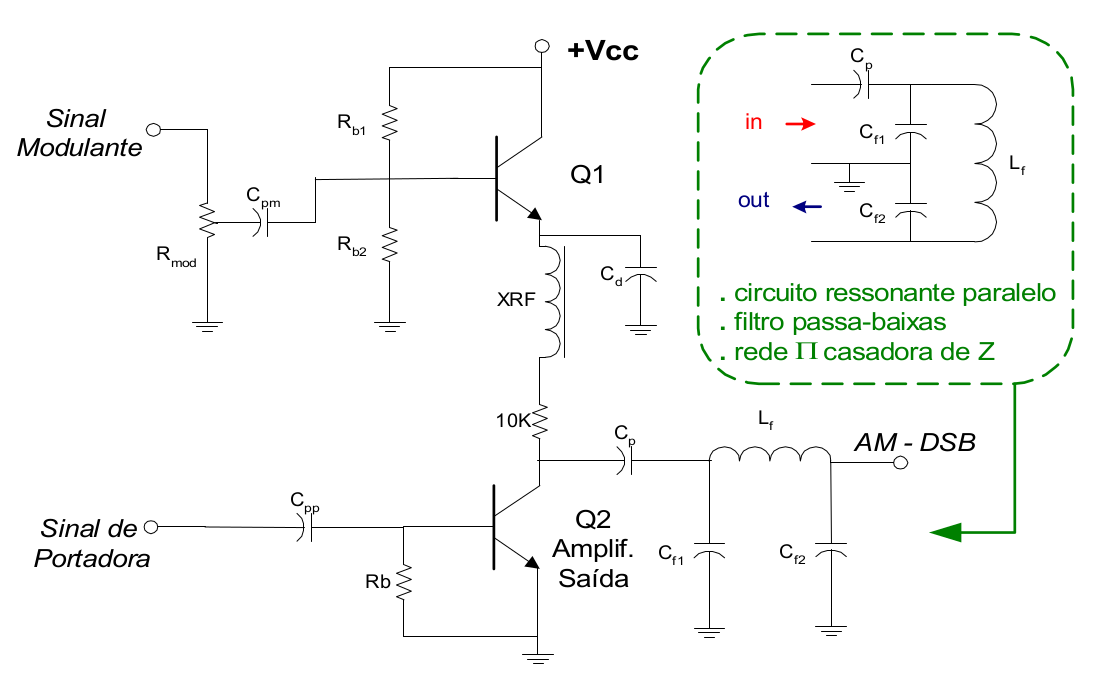
\includegraphics[scale=0.4]{Imagens/mod_am_serie.png}
    \label{f_mod_am_serie}
\end{figure}

\subsubsection{Modulador a diodo}

A figura \ref{f_mod_am_diodo} apresenta a configuração do circuito utilizado em um modulador AM/DSB simples.
Os moduladores série modificam diretamente a amplitude do sinal de RF, assim, evitando distorções na frequência do sinal modulado.

\begin{figure}[H]
    \centering
    \caption{Circuito do modulador a diodo.}
    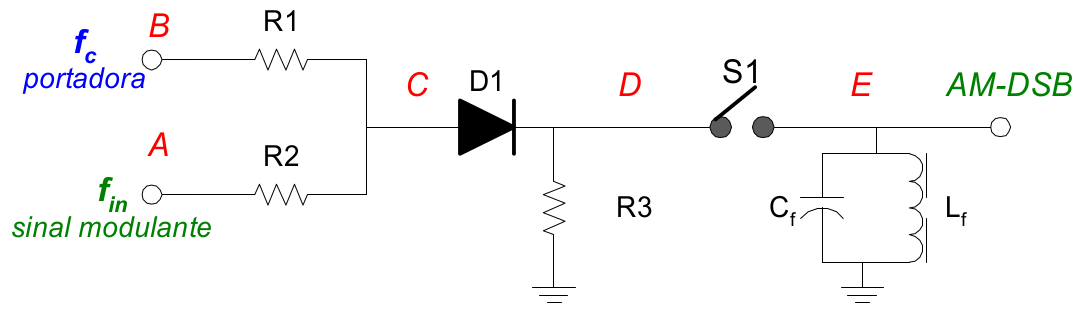
\includegraphics[scale=0.4]{Imagens/mod_am_diodo.png}
    \label{f_mod_am_diodo}
\end{figure}

A chave S1, quando o circuito está em operação, fica normalmente fechada.
O filtro passa-faixa composto por $C_f$ e $L_f$ é sintonizado em $f_c$. Assim, para cada semi-ciclo positivo de $f_c$ o circuito ressonante paralelo produz um semi-ciclo negativo, resultando à saída a forma de
onda E da figura \ref{f_mod_am_diodo_ex}.



\begin{figure}[H]
    \centering
    \caption{Formas de onda em um modulador a diodo.}
    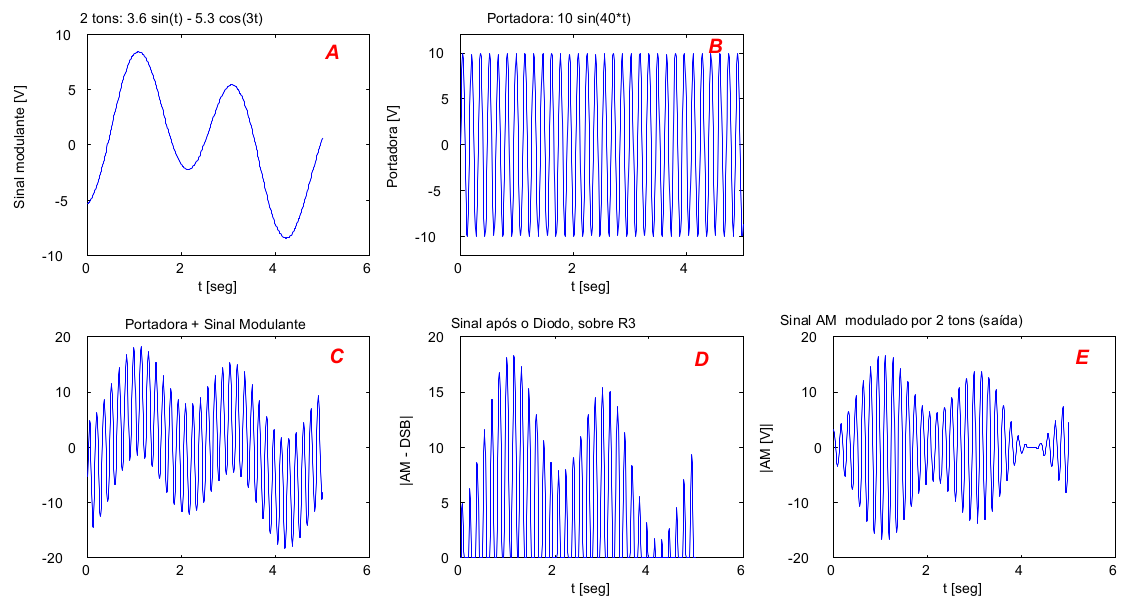
\includegraphics[scale=0.4]{Imagens/mod_am_diodo_ex.png}
    \label{f_mod_am_diodo_ex}
\end{figure}